\documentclass[a4paper]{article}

%% Font selection
\usepackage{DejaVuSerifCondensed, DejaVuSansCondensed, DejaVuSansMono}
\usepackage{microtype}
\usepackage[T1]{fontenc}

%% Listings (see https://www.ctan.org/pkg/minted for installation)
\usepackage[outputdir=.texpadtmp]{minted}
\setminted{fontsize=\small, frame = leftline, framesep = 2\fboxsep}
\setmintedinline{ fontsize=\normalfont }
\usepackage{upquote}  % TT quotes in listings

%% Other packages
\usepackage[english]{babel}  % Language support
\usepackage{lipsum}  %TODO REV Remove
\usepackage{graphicx, epstopdf}  % Support EPS figures
\epstopdfsetup{outdir=.texpadtmp/}
\usepackage{url, hyperref}  % \url command, properly working
\usepackage[style=alphabetic]{biblatex}  % Bibliography
\addbibresource{bibliography.bib}
 
%% Shortcuts
\usepackage{xspace}
\newcommand{\matlab}{\textsc{Matlab}\xspace}
\newcommand{\csv}{\texttt{CSV}\xspace}

%% Last package of all
\usepackage{cleveref}  % Allows en­hanced cross-ref­er­enc­ing fea­tures

%% Document details
\title{Piecewise segmentation for financial data}
\author{Paolo Antonini \and Davide Azzalini \and Fabio Azzalini}
\date{}

%% DOCUMENT
\begin{document}

\maketitle

\begin{abstract}
Time series data is characterised as large in data size, high dimensionality and update continuously. Moreover, the time series data is always considered as a whole instead of individual numerical fields. As a consequence, in order to analyse and mine time series data, segmentation and dimensionality reduction are essential. In particular, in the following pages we are going to collect and study some segmentation methods, applied in particular to stock market data. Stock time series has its own characteristics over other time series. 
\end{abstract}

\section{Introduction}
The tasks of segmentation and dimensionality reduction, as well as identification of trends, are fundamental to allow a number of time series analysis and mining tasks. As a matter of fact, the fields of application of such procedures are numerous (ECG, exchange rates, sensor detections of any kind, \dots) and methods differ from application to application, due to the characteristics of data. As a consequence, literature regarding these issues is vast. 

In particular, our focus is on stock market data, which is inherently large in size, noisy and continuously updated. In this paper we are going first to list some of the main research papers where dimensionality reduction and piecewise segmentation are studied, in \cref{sec:methods}. Then, in \cref{sec:implementations} we are going to present some implementations of the methods. 


\section{Methods}\label{sec:methods}
\lipsum[1]

\subsection{\citeauthor{5961935}. \citetitle{5961935}}
\lipsum[2-3]


\section{Implementations}\label{sec:implementations}

\lipsum[7]

\subsection{Turning points in \matlab}

Here we are presenting our implementation of the method to find \emph{turning points}, as it was presented in \cite{5961935}.%TODO REV Check bibliography.

The method is developed and tested over \csv files downloaded from Yahoo! Finance website\footnote{\url{http://finance.yahoo.com/market-overview/}}. Should another source be used, basic adaptations may be necessary, mostly in the handling of temporal data\footnote{Due to our limited knowledge of Matlab language, we may have dealt with this kind of data in a na{\"i}ve way.} (i.e., dates). 

After importing the aforementioned \csv file (we suggest to use the graphical interface provided by \matlab itself), the user should issue the following command, in order to compute and plot the results: \mint{matlab}{y = TurningPoints(Date, Close, 1);}

\texttt{TurningPoints()} function is implemented as shown in \cref{lst:turningPoints}, with the support of some side functions. We will not analyse the theoretical details of the algorithm, as they are covered in our reference document.

\begin{listing}[H]
 
\inputminted[firstline = 1, lastline = 50]{matlab}{../code/TurningPoints.m}

\caption{\texttt{TurningPoints()} function.}\label{lst:turningPoints}

\end{listing}

The main supporting function is \texttt{TP\_preprocess()}, which implements the very first part of the algorithm in \cite{5961935}, and is presented in \cref{lst:preprocess}. The other supporting functions are of secondary importance, so we are not presenting them here. Basically we have: \begin{itemize}
	\item \texttt{TP\_prepareData()} takes in input raw Yahoo! Finance data and prepares it for being processed;
	\item \texttt{TP\_cleaning()} cleans data matrix after processing;
	\item \texttt{TP\_output()} shows information about the processing (i.e., the number of deleted elements).
\end{itemize} 

\begin{listing}[H]
 
\inputminted[firstline = 53, lastline = 78]{matlab}{../code/TurningPoints.m}

\caption{\texttt{TP\_preprocess()} supporting function.}\label{lst:preprocess}

\end{listing}


To conclude our discussion, we are presenting some tests we performed. Weekly stock market data from A2A (\texttt{A2A.MI}) over the whole 2015 was used as source. In \cref{fig:a2a_w_2015} we show the original data in blue, the preprocessed data in orange and the data after one full run of the algorithm in yellow. % TODO REV Check cross-reference.

\begin{figure}[H]
	
	\makebox[\textwidth][c]{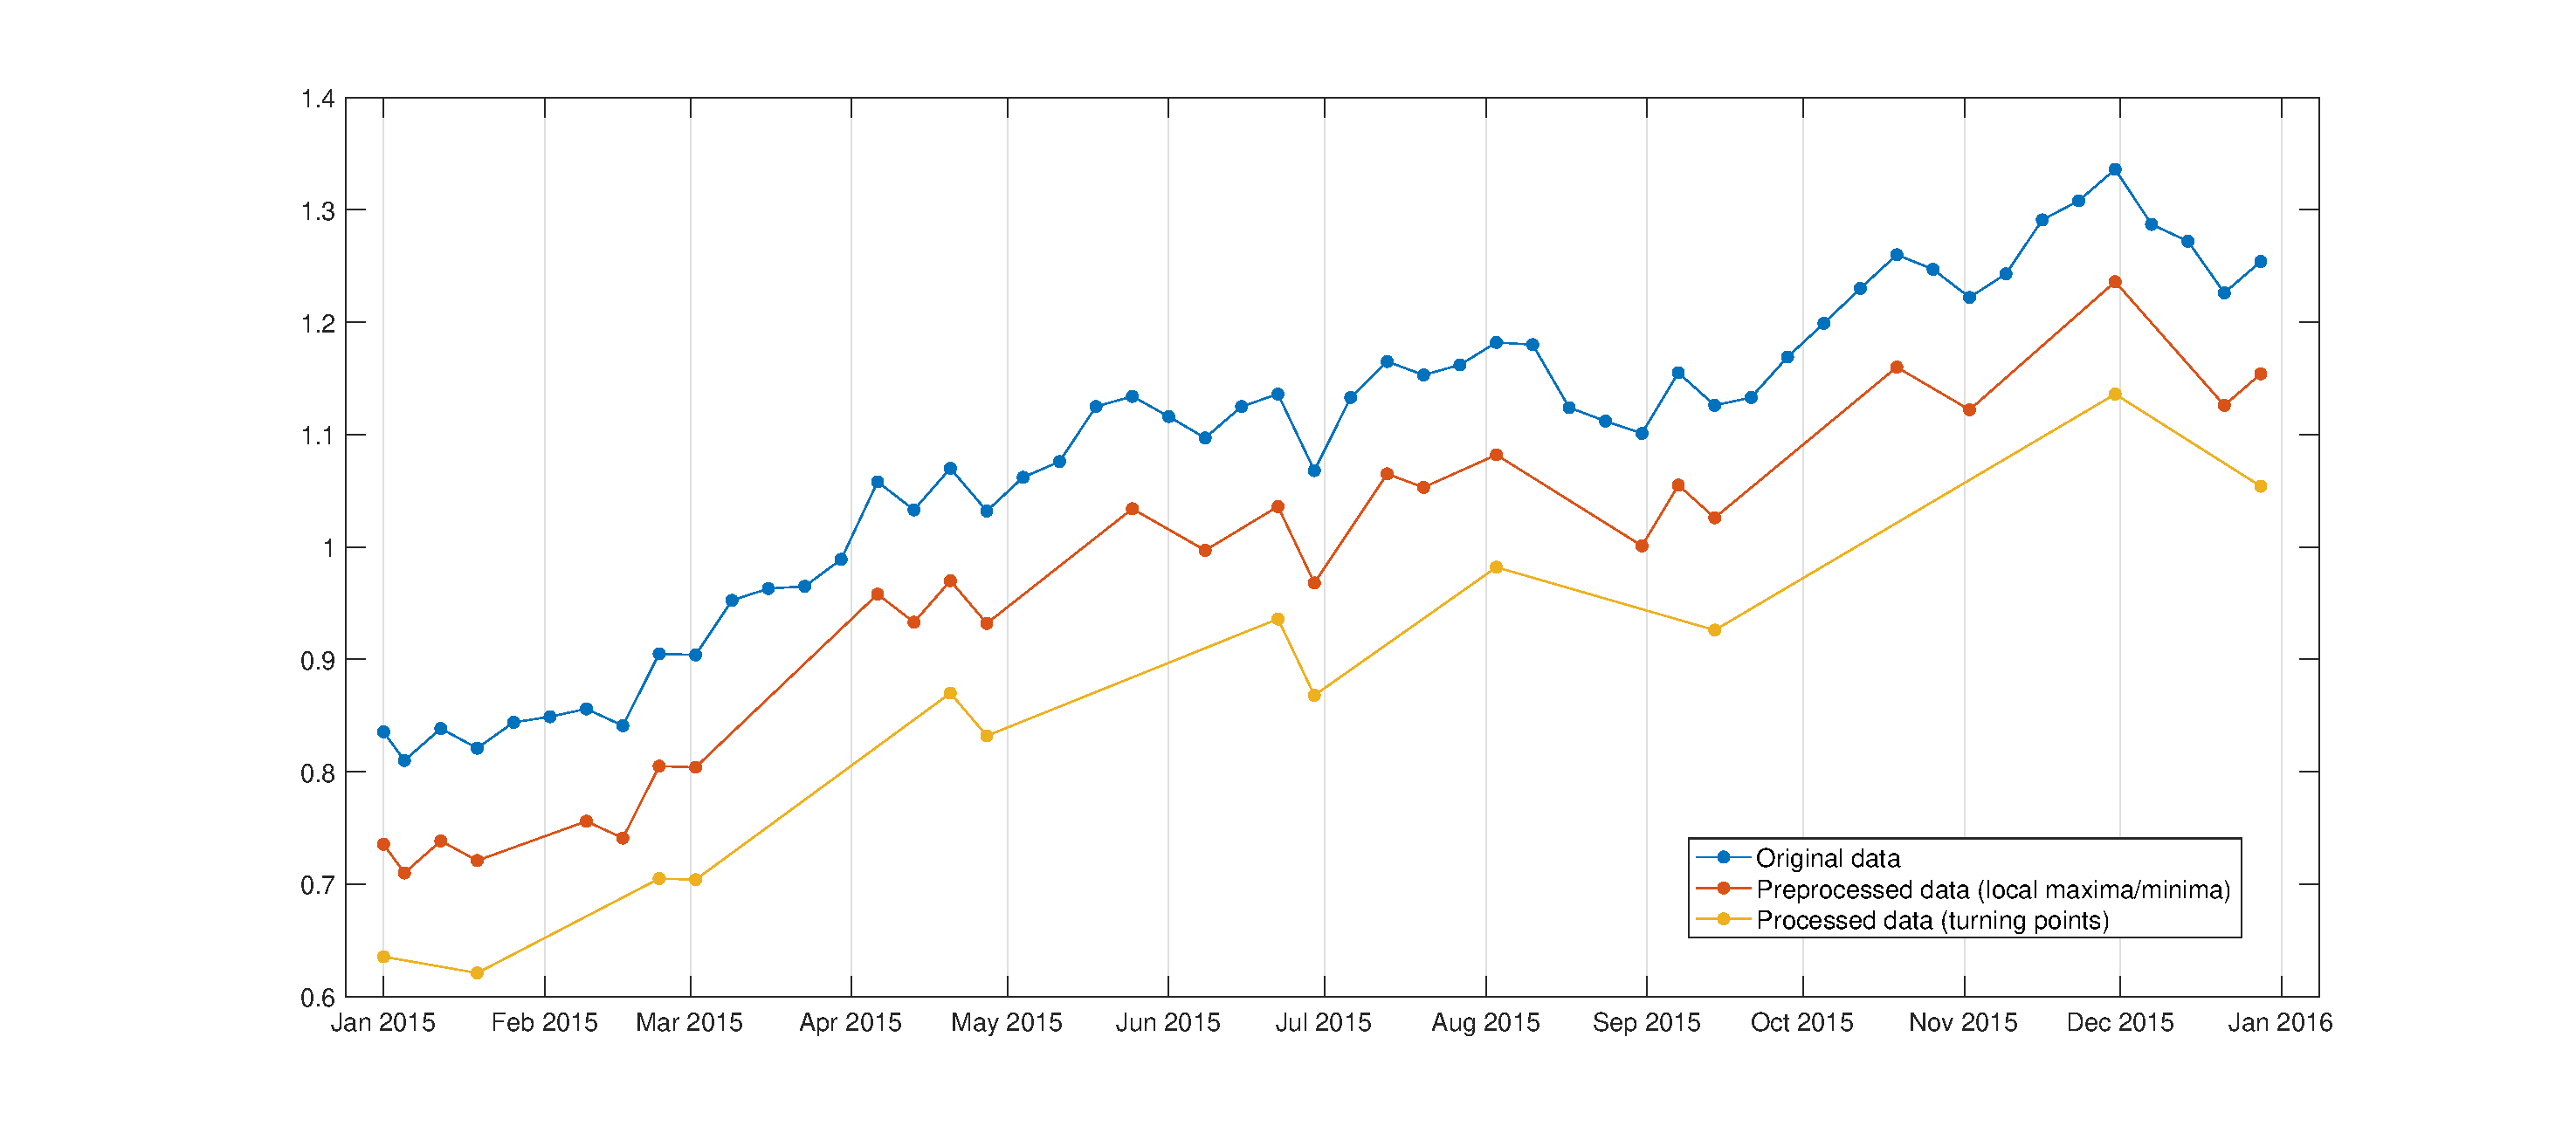
\includegraphics[width=1.8\textwidth]{img/a2a_W_15}}
	
	\caption{\texttt{A2A.MI} weekly 2015. Original data (53 samples) is in the correct position. The other two series (respectively 27 and 12 samples) are shifted down by 0.1 each.}
	
	\label{fig:a2a_w_2015}

\end{figure}


\subsection{Other implementations} 
\lipsum[4-6]


%TODO Sistema.
\defbibnote{prenote}{DOI, when defined, serves as URL to retrieve the document. Documents may be accessible only on institutional log in (e.g., academic credentials).}
\printbibliography[title={Bibliography}, prenote=prenote]


\end{document}







